%========= Introduction
\section{Introduction}
\label{sec:introduction}

In the complex and ever-evolving world of \ac{EW}, quantum computing could provide the ability to understand radar signals in novel ways, never before seen in this field. 
It is widely recognised in the discipline of electronic warfare that traditional signal analysis techniques are still bounded by computational constraints, so in order to maintain strategic advantage, new techniques are continuously needed in order to keep pace with emerging threats. 
Quantum computing may promise a paradigmatic shift in extracting actionable insights from massive and complex \ac{EW} datasets. 

Recent research has demonstrated a great potential for quantum computing to address the challenges of modern signal processing
\cite{somma_quantum_2019, daskin_walk_2022},
however little work has been devoted to its applications in \ac{EW} signal processing, and more specifically radar signal processing 
Therefore, this report explores the question of how quantum technology may be applied
to radar signal processing in EW
At first, a survey of the current state of research will be conducted for radar signal analysis and quantum signal processing. 
Then, an empirical inquiry into the subject will be presented, aiming to determine 
how quantum methods can be used to encode, characterise, and de-interleave radar signals.
Finally, a discussion of results, examination of limitations, and consideration for future work will be provided. 
 
Despite quantum computing holding much promise, its potential in this field remains largely unexplored. This report will present a background and preliminary investigation into how quantum computing can be utilised in the dynamic landscape of electronic warfare. 

\subsection{Background}~\label{subsec:background}

Radar is "an electrical system that transmits \ac{RF} \ac{EM} waves toward a region of interest and receives and detects these EM waves when reflected
from objects in that region."\cite{richards_principles_2010}. The name radar originates from a portmanteau of \textit{Radio Detection and Ranging}\cite{the_joint_board_on_scientific_information_policy_radar_1945}, hinting at it's founding objectives in the defence context. In the modern day, radar is used in many civilian and military applications \cite{merrill_i_skolnik_radar_nodate, desai_how_2022}:
\begin{itemize}
    \item Aerospace - weather, navigation, approach, altitude, identification
    \item Maritime - navigation, collision avoidance,  
    \item Ground Penetrating - archaeology, mining, oceanographic sounding
    \item Space - spacecraft and celestial monitoring
    \item Automotive - civilian and law enforcement
    \item Industrial - fluid sensing, speed measurement
    \item Medical
    \item Atmospheric / Weather
    \item Electronic Warfare
\end{itemize}

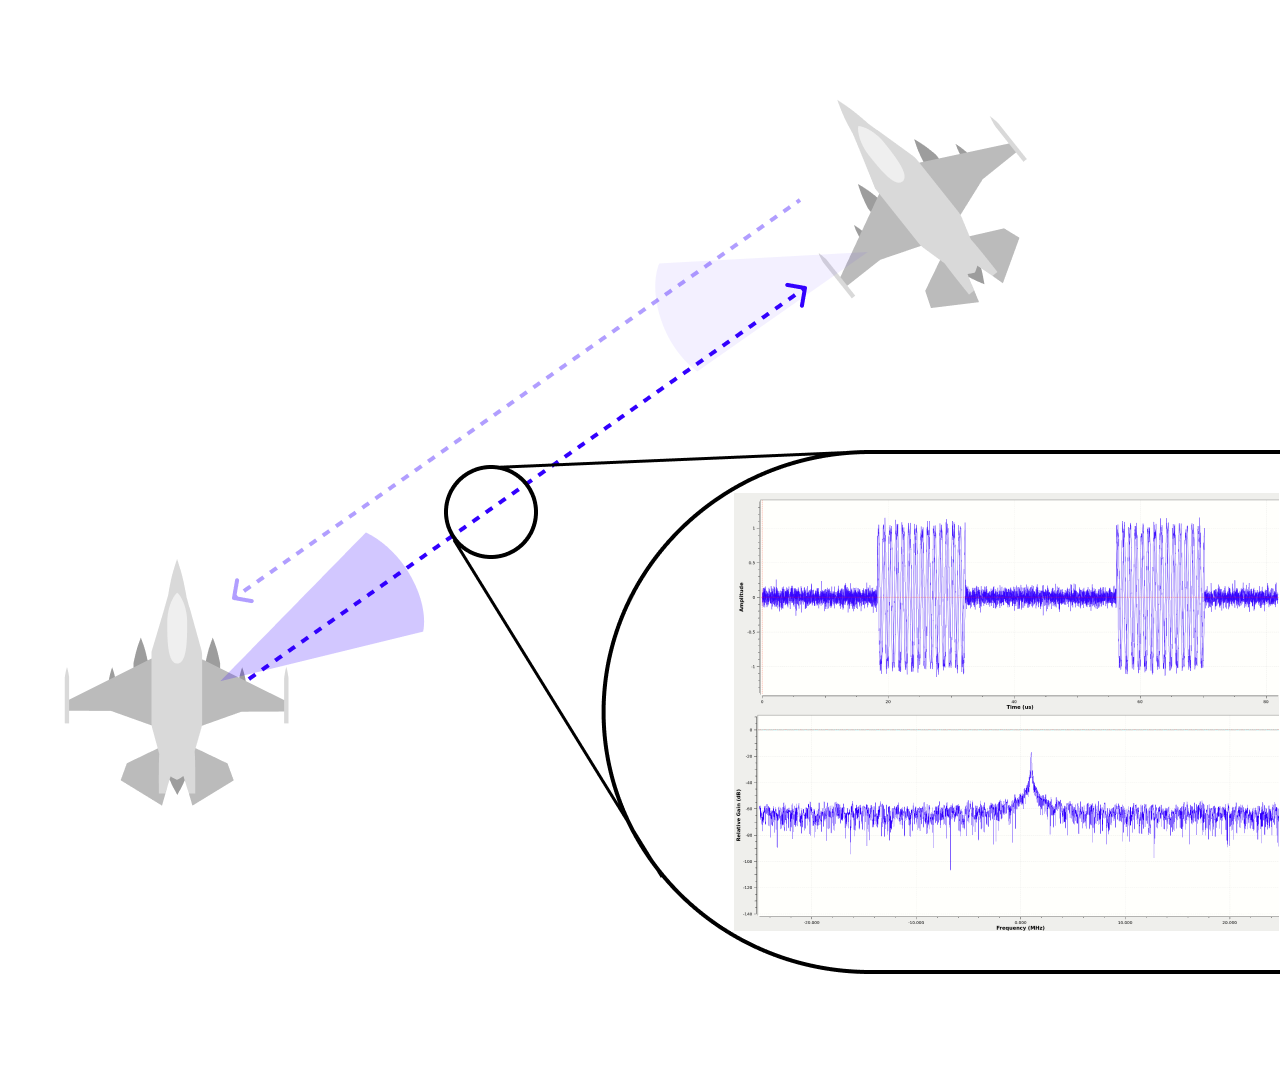
\includegraphics[width=\textwidth]{Figures/Senario_ Single Radar; single signal.png}

Since radar systems were invented in 1930 \cite{degering_invention_2018}, their usage has become increasingly widespread. As a result, the electromagnetic environment has become densely populated, with a multitude of different emitters posing a challenge of unintentional interference with operating radars \cite{degering_invention_2018}. However, their widespread adoption - particularly in the defence context - yields the potential to identify the location and type of emitters in the area of operation.\todo{Passive; ESM}
This subject has been encompassed in the broader discipline of \ac{EW}. \ac{EW} is defined by David Adamy \cite{adamy_13_2001} as "the art and science of preserving the use of the electromagnetic spectrum for friendly use while denying its use to the enemy"\todo{I think a different definition would be best here, or perhaps referencing ELINT...}.

\ac{ESM}, a sub-field of \ac{EW}, where \ac{ESM} as "the receiving part of EW"\cite{adamy_13_2001}, of which radar is the principal element".

\todo{Describe the importance of radar \ac{ESM} here. Who cares and why? }

\todo{Principles of radar}

A typical radar system is made up of at least one of each: radio transmitter, radio receiver, antenna, and display \cite{stimson_introduction_1998}. % There was a more precise definition somewhere with a 'signal processor' element.

% The ESM pipeline
% IQ Data -> Pulse Detection -> Pulse Compression -> Doppler Processing -> Constant False Alarm Rate (CFAR) Detection -> Target Association -> Tracking -> Classification -> Decision

% ------------
% BELOW IS A GENERAL OUTLINE. It highlights the sequence of radar processing.
% ------------
% Pulse Detection:
% - Matched filtering or other pulse detection algorithm to identify radar pulses
% - Thresholding to remove noise and false detections

% Pulse Compression:
% - Matched filtering or other pulse compression algorithm to enhance SNR of pulses
% - Windowing to reduce sidelobes and improve spectral properties

% Doppler Processing:
% - Fourier transform or other Doppler processing algorithm to estimate target velocity
% - Doppler filtering to reject clutter and interference

% CFAR Detection:
% - CFAR algorithm to detect targets in the presence of noise and clutter
% - Adaptive thresholding to adjust detection threshold based on local noise level

% Target Association:
% - Clustering or other target association algorithm to group detections into tracks
% - Filtering or smoothing to reduce track jitter and improve accuracy

% Tracking:
% - Kalman filter or other tracking algorithm to predict target state and estimate measurement errors
% - Maneuver detection and tracking to handle agile targets

% Classification:
% - Feature extraction and classification algorithm to identify target type
% - Machine learning or rule-based classification

% Decision:
% - Target prioritization and threat assessment
% - Decision making based on mission objectives and rules of engagement
% - Display and dissemination of results
% ------------------------------

\todo{Link back to:\ac{ESM} \ac{ECM} \ac{ECCM}. Here, consider providing a precise definition of \ac{ESM}. Also, somewhere here, a mention of \ac{ELINT} should be made}

For the radar to achieve its objectives, it must be able to convert observed data into actionable information, thereby requiring some degree of information processing. Herein lies the general challenges in \ac{ESM} - the detection, location, and identification of targets, which will now be explored. % Cite 'detection, location and identification' - I think the precise term is 'analysis'.

First, however, a conceptual schematisation of this system must be made in in terms of its inputs, process, and outputs. In \ac{ESM}, inputs consist of EM fluctuations that vary over time. They are almost always received by an antenna (or antennas) which may be subsequently manipulated in the analogue and digital domains. These fluctuations, henceforth \textit{signals} (not to be confused with communications signals), are the essential information carriers in the signal processing operation. There also exist inputs derived from the nature of the radar system configuration itself. These may include the antenna configuration and receiver architecture which will not here be considered, but is noted by the author as being of significant relevance to kinematic measurement and capability constraints.

Since the signals of interest are those emitted by radar systems, the received signals exhibit phenomenal qualities corresponding to those of the originating radar, namely: \cite{avionics_department_electronic_2013} 5-8.1
\begin{itemize}
    \item Frequency (\ac{RF}): Intrapulse frequency, modulation (and associated modulation parameters); Interpulse: phase coherence.
    \item Amplitude (power)
    \item \ac{DOA} / \ac{AOA}
    \item \ac{TOA}
    \item \ac{PRI}, \ac{PRF}
    \item \ac{PRI} type
    \item \ac{PW}
    \item Scan type and rate
    \item Lobe duration (beam width or dwell)
\end{itemize}

The role of the processing step, is to convert the 'raw' signal into these parameters. Optimally, the parameters equal those nominally transmitted by the target radar.
These are generally extracted from the incident \ac{EM} signals and may be treated independently as outputs themselves. Typically, however, further analysis may be may conducted to yield very granular information. Information that \ac{ESM} seeks to understand addresses many facets:
\begin{itemize}
    \item Detection
    \item Target characteristics \cite{jenn_radar_2007}
    \begin{itemize}
        \item target size - return amplitude
        \item target shape - from discrete scan returns
        \item target material composition
        \item moving parts (modulation of the return)
    \end{itemize}
    \item Target identification
    \item Kinematic parameters and tracking(range, direction, speed, \ac{AOA})
\end{itemize}

\todo{Introduce multi-radar concept. }
\todo{Illustrate a scenario to make the problem more evident.}

\subsubsection{Research Question}
% To what extent can quantum computing methods can quantum computing be used to understand radar signals?
How can quantum computing methods be used to in an ESM function to detect the types and characteristics of radar signals in the defence context?

\subsubsection{Research Objectives}
\begin{itemize}
    \item Acquire a source data emulator to be used to test and verify quantum implementations.
    \item Identify the specific types of radar signals used in radar systems and their key signal parameters, based on an analysis of publicly available technical documents and datasets.
    \item Develop a quantum-based encoding method that converts sampled time-domain radar signals into qubits.
    \item Validate the quantum encoding method by evaluating the expressivity, complexity, and qualitative suitability.
    \item Develop a method for quantum-based pulse detection of a radar signals that vary in type and quality. The method must be quantifiably measurable.
    \item Validate the quantum pulse detection method by evaluating the accuracy of pulse boundary detection and signal-to-noise tolerance.
    \item Determine a quantum method for estimating a radar signal's frequency.
    \item Validate the frequency estimation method by evaluating the accuracy and signal-to-noise tolerance.
\end{itemize}

\subsection{Scope}

\subsubsection{Out of Scope}

\todojc{This section may need some initial statement and each bullet point some brief explanation}\begin{itemize}
    \item Hardware
        No consideration of hardware constraints 
    \item Anything down-stream of identification of radar signals. (e.g., display, databasing, data fusion, etc.)
    \item \ac{SAR} and antenna-specific computation (i.e., bistatic/multistatic antenna setups)
    \item Imaging
    \item Kinetic estimation (range, velocity, angle of arrival, etc.)
    \item Forecasting
    \item Active emission.
    \item Simulation / emulation
    \item Radio signals only; sub-millimetre-wave technology is not considered.
    \item Resource allocation
    \item Ambiguity analysis
    \item Tracking
    \item Multipath effects
\end{itemize}

% Identify the challenge with multi-radar environments.

% Provide a brief outline of the genus of classical processing approaches.\
% Introduce quantum computing, and provide an abstracted overview of its potential application to this field.
% Conclude the case for quantum computing in ESM. Providce an implicit definition of the research question
% Identify the challenges with quantum computing.

\begin{quote}
    \textit{"The increased pulse density created by the deployment of pulse Doppler radar, both enemy and friendly, has created demand for systems with a high signal processing capability"} \cite{pettersson_illustrated_1992} p. 42
\end{quote}


% ---------------
% OLD EXPLANATION
% ---------------
% One category of radar is pulsed-Doppler which emits energy in high-frequency pulses. The characteristics of the pulses impact the range resolution, with shorter pulses allowing for higher resolution because the receive signal is too shorter. However, the trade-off is that a shorter pulse means less time for the emission to illuminate the target, and therefore less return amplitude and shorter maximum range. One way to counter this issue is to use a technique named ‘pulse compression’. In principle, the technique bypasses this limitation by transmitting infinitely short pulses. How? By means of frequency modulation; by ramping the transmission frequency linearly up or down. The difficulty is: how to receive a single pulse over these many frequencies. The solution is in using an analogue filter with a non-linear phase response which causes lower frequencies to be ‘delayed’ or phase-shifted, more than higher frequencies, In effect it ‘compresses’ the returned pulse into a higher power pulse, thereby increasing both range resolution, and maximum range. This, however, is not enough. Higher range and resolution are desired – and that means more power! A single pulse is alone insufficient in solving the problem; the solution lays in multiple pulses. By sending more than one pulse, one increases the average transmitted power on the target (and thus returns). With multiple pulses, the chances of a return being intercepted are increased. These pulses must be transmitted consecutively therefore, at some Pulse Repetition Frequency (PRF). However effective upon first thought, a limitation always arises – range ambiguity. If a pulse is transmitted and, before the its return received, another pulse arrives,  \cite{parker_chapter_2010}

% --------------
% OLD OBJECTIVES
% --------------
% In the processing functional block, the problems for radar are, in sequential order:
% \begin{itemize}
%     \item How to distinguish between the different categories of signals: communications, interference, radar, and noise.
%     \item Then, after having understood what signals are radar intercepts, identifying which belong to the same originating receiver. 
%     \item Once, a radar signal has been de-interleaved, how to identify the originating emitter, given some a priori understanding of the operational environment.
% \end{itemize}
% \begin{itemize}
%     \item To further understand the principles of operation of passive radar systems, including their ability to detect and identify emitters in complex electromagnetic environments.
%     \item To critically evaluate existing literature on radar systems and quantum computing to effecively communicate existing the academic knowledge, and to show a capability to conduct independent future research.
%     \item To identify the possibilities of using Quantum Computing in Radar signal analysis; to also identify three candidate avenues; to explore one in enough depth to evaluate potential feasability though the creation of a technical solution
%     \item To prioritize research topics based on their level of desirability and feasibility, and to develop a plan for executing research projects within a defined timeline and scope.
%     \item To communicate research findings effectively to a technical audience.
% \end{itemize}
% \begin{itemize}
%     \item Identify a candidate method, or methods for converting continuously varying parameterised radar signals into into discrete radar modes using quantum methods?
%     \item Is it possible, and to what extent are quantum methods effective in de-interleaving and signal clustering?
%     \item Can quantum computing effectively track a radar signal intercept, and how well?
%     \item %\almarginpar{Would the last two-four be in too hard basket for the time frame? May be better to leave those for the motivation section - if we could do the previous then we'd be able to do the following?}
%     In the radar context, can, and how well are quantum computing methods disposed to help in reducing noise, interference, and clutter?
% \end{itemize}
